\documentclass[tikz,border=10pt]{standalone}
\usepackage{amsmath}
\usetikzlibrary{positioning, arrows.meta, calc, shapes}

% Define colors
\definecolor{attnblue}{RGB}{100,150,255}
\definecolor{ffnorange}{RGB}{255,180,100}
\definecolor{normgreen}{RGB}{120,220,120}
\definecolor{maskred}{RGB}{255,100,100}

\begin{document}

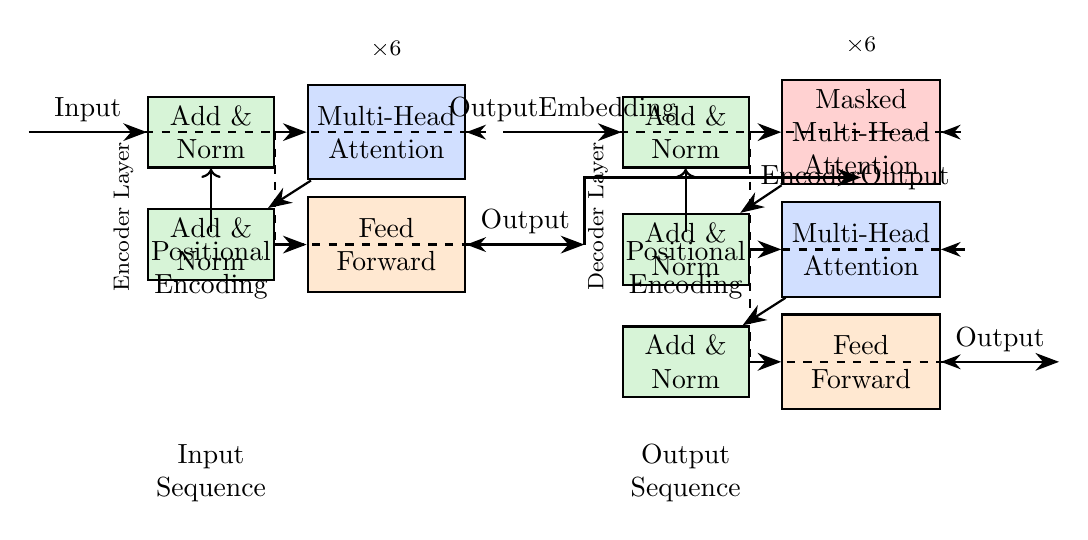
\begin{tikzpicture}[
    block/.style={rectangle, draw, thick, minimum height=1.2cm, minimum width=2cm, align=center},
    smallblock/.style={rectangle, draw, thick, minimum height=0.8cm, minimum width=1.6cm, align=center},
    arrow/.style={-{Stealth[length=3mm]}, thick},
    dashedarrow/.style={-{Stealth[length=2.5mm]}, dashed, thick}
]

% === ENCODER STACK ===
\node[block, fill=attnblue!30] (enc_attn) {Multi-Head \\ Attention};
\node[block, below=0.2cm of enc_attn, fill=ffnorange!30] (enc_ffn) {Feed \\ Forward};
\node[smallblock, left=0.4cm of enc_attn, fill=normgreen!30] (enc_norm1) {Add \& \\ Norm};
\node[smallblock, left=0.4cm of enc_ffn, fill=normgreen!30] (enc_norm2) {Add \& \\ Norm};

% Encoder connections
\draw[arrow] ([xshift=-1.5cm]enc_norm1.west) -- (enc_norm1.west) node[midway, above] {Input};
\draw[arrow] (enc_norm1) -- (enc_attn);
\draw[arrow] (enc_attn) -- (enc_norm2);
\draw[arrow] (enc_norm2) -- (enc_ffn);
\draw[arrow] (enc_ffn) -- ([xshift=1.5cm]enc_ffn.east) node[midway, above] {Output};

% Residual connections (dashed)
\draw[dashedarrow] ([xshift=-1.5cm]enc_norm1.west) |- ($(enc_attn.east)+(0.3,0)$) -- (enc_attn.east);
\draw[dashedarrow] (enc_norm1.east) |- ($(enc_ffn.east)+(0.3,0)$) -- (enc_ffn.east);

% Encoder stack label
\node[rotate=90, left=0.3cm of enc_norm1, font=\footnotesize] {Encoder Layer};
\node[above=0.2cm of enc_attn, font=\footnotesize] {×6};

% === DECODER STACK ===
\node[block, right=4cm of enc_attn, fill=maskred!30] (dec_mask_attn) {Masked \\ Multi-Head \\ Attention};
\node[block, below=0.2cm of dec_mask_attn, fill=attnblue!30] (dec_attn) {Multi-Head \\ Attention};
\node[block, below=0.2cm of dec_attn, fill=ffnorange!30] (dec_ffn) {Feed \\ Forward};

\node[smallblock, left=0.4cm of dec_mask_attn, fill=normgreen!30] (dec_norm1) {Add \& \\ Norm};
\node[smallblock, left=0.4cm of dec_attn, fill=normgreen!30] (dec_norm2) {Add \& \\ Norm};
\node[smallblock, left=0.4cm of dec_ffn, fill=normgreen!30] (dec_norm3) {Add \& \\ Norm};

% Decoder input
\draw[arrow] ([xshift=-1.5cm]dec_norm1.west) -- (dec_norm1.west) node[midway, above] {Output \\ Embedding};

% Decoder internal flow
\draw[arrow] (dec_norm1) -- (dec_mask_attn);
\draw[arrow] (dec_mask_attn) -- (dec_norm2);
\draw[arrow] (dec_norm2) -- (dec_attn);
\draw[arrow] (dec_attn) -- (dec_norm3);
\draw[arrow] (dec_norm3) -- (dec_ffn);
\draw[arrow] (dec_ffn) -- ([xshift=1.5cm]dec_ffn.east) node[midway, above] {Output};

% Decoder residual connections
\draw[dashedarrow] ([xshift=-1.5cm]dec_norm1.west) |- ($(dec_mask_attn.east)+(0.3,0)$) -- (dec_mask_attn.east);
\draw[dashedarrow] (dec_norm1.east) |- ($(dec_attn.east)+(0.3,0)$) -- (dec_attn.east);
\draw[dashedarrow] (dec_norm2.east) |- ($(dec_ffn.east)+(0.3,0)$) -- (dec_ffn.east);

% Cross-attention from encoder
\draw[arrow] ([xshift=1.5cm]enc_ffn.east) |- ([yshift=0.3cm]dec_attn.north) node[pos=0.8, right] {Encoder \\ Output};

% Decoder stack label
\node[rotate=90, left=0.3cm of dec_norm1, font=\footnotesize] {Decoder Layer};
\node[above=0.2cm of dec_mask_attn, font=\footnotesize] {×6};

% === POSITIONAL ENCODING ===
\node[below=0.8cm of enc_norm1, align=center] (pe_enc) {Positional \\ Encoding};
\node[below=0.8cm of dec_norm1, align=center] (pe_dec) {Positional \\ Encoding};

\draw[->, thick] (pe_enc) -- ++(0,0.6) -| (enc_norm1.south);
\draw[->, thick] (pe_dec) -- ++(0,0.6) -| (dec_norm1.south);

% === INPUT/OUTPUT LABELS ===
\node[below=1.6cm of pe_enc, align=center] {Input \\ Sequence};
\node[below=1.6cm of pe_dec, align=center] {Output \\ Sequence};

\end{tikzpicture}

\end{document}
